\documentclass[11pt]{article}
\usepackage[T1]{fontenc}
\usepackage[utf8]{inputenc}
\usepackage[letterpaper]{geometry}

\usepackage{graphicx}
\usepackage{mathpazo}

\usepackage{amsmath}
\usepackage{amsfonts}
\usepackage{bm}
\usepackage{siunitx}
\usepackage{cancel}
\usepackage{float}
\usepackage{empheq}
\usepackage[most]{tcolorbox}

% Sexy yellow highlighted boxed equations!
\newtcbox{\mymath}[1][]{%
	nobeforeafter, math upper, tcbox raise base,
	enhanced, colframe=black!30!black,
	colback=yellow!30, boxrule=1pt,
	#1}

% Hyperlinks with decent looking default colors.
\usepackage{hyperref}
\usepackage{xcolor}
\hypersetup{
	colorlinks,
	linkcolor={red!50!black},
	citecolor={blue!50!black},
	urlcolor={blue!80!black}
}

% For those sexy spaced low small caps from classic-thesis!
\usepackage{microtype}
\usepackage{textcase}
\DeclareRobustCommand{\spacedlowsmallcaps}[1]{%
	\textls[80]{\scshape\MakeTextLowercase{#1}}%
}

% Replaced mathpazo \sum symbol with computer modern's.
\DeclareSymbolFont{cmlargesymbols}{OMX}{cmex}{m}{n}
\let\sumop\relax
\DeclareMathSymbol{\sumop}{\mathop}{cmlargesymbols}{"50}

% Force indent command.
\newcommand{\forceindent}{\leavevmode{\parindent=1em\indent}}

% Math shortcuts.
\newcommand\p[2]{\frac{\partial #1}{\partial #2}}

% fancyhdr header and footer.
\usepackage{fancyhdr}
\pagestyle{fancy} 
\fancyhead{}
\rhead{Ali Ramadhan}
\chead{}
\lhead{12.818: Project 5}
\cfoot{}
\rfoot{\thepage}

\title{\spacedlowsmallcaps{\small 12.818: Introduction to Atmospheric Data and Large-scale Dynamics}\\ \spacedlowsmallcaps{\Large Project five: Geostrophic and ageostrophic flow}}
\author{\spacedlowsmallcaps{Ali Ramadhan}}
\date{}

% \renewcommand\thesection{\Alph{section}}

\begin{document}
\maketitle

To a rough first approximation, the wind patterns we observe daily can be explained to result from the balance between the Coriolis force ($2\bm{\Omega \times u}$ per unit mass) due to the Earth's rotation and the pressure gradient force ($\nabla p / \rho$). An identical balance can be found in the ocean as well. In pressure coordinates it can mathematically be stated as
\begin{subequations}
\begin{align}
	v &= \frac{g}{f} \frac{\partial h}{\partial x} \label{eq:1v} \\
	u &= -\frac{g}{f} \frac{\partial h}{\partial y} \label{eq:1u}
\end{align}
\end{subequations}
where $\bm{u} = (u,v)$ is the velocity field or wind speed, $h(x,y)$ is the geopotential height map at a constant pressure level, $g = \SI{9.81}{\m/\s^2}$ is the acceleration due to gravity, commonly taken to be constant, and $f=2\Omega \sin\phi$ is the \emph{Coriolis parameter} where $\Omega = \SI{7.29e-5}{\radian/\s}$ is the angular rotation rate of the Earth and $\phi$ is the latitude coordinate.

In this project we will look at how accurately geostrophic balance holds for the atmosphere in a few different cases.

\section{Geostrophic wind}
Figure \ref{fig:hudson} shows the geopotential height of the \SI{500}{\hecto\Pa} constant pressure surface over the northern United States and Canada on October 12, 2017 0Z. We would like to make a crude estimate of the geostrophic wind at a point and compare it with the observed wind speed. We will do this for the southeastern corner of the Hudson Bay at the \SI{5530}{\m} geopotential height contour. As the geopotential height contours are approximately parallel to the lines of latitude at this particular time, we would expect the geostrophic wind to maintain an east-west $u$-component which we will estimate using Eq. \eqref{eq:1u}.

\begin{figure}[h!]
	\centering
	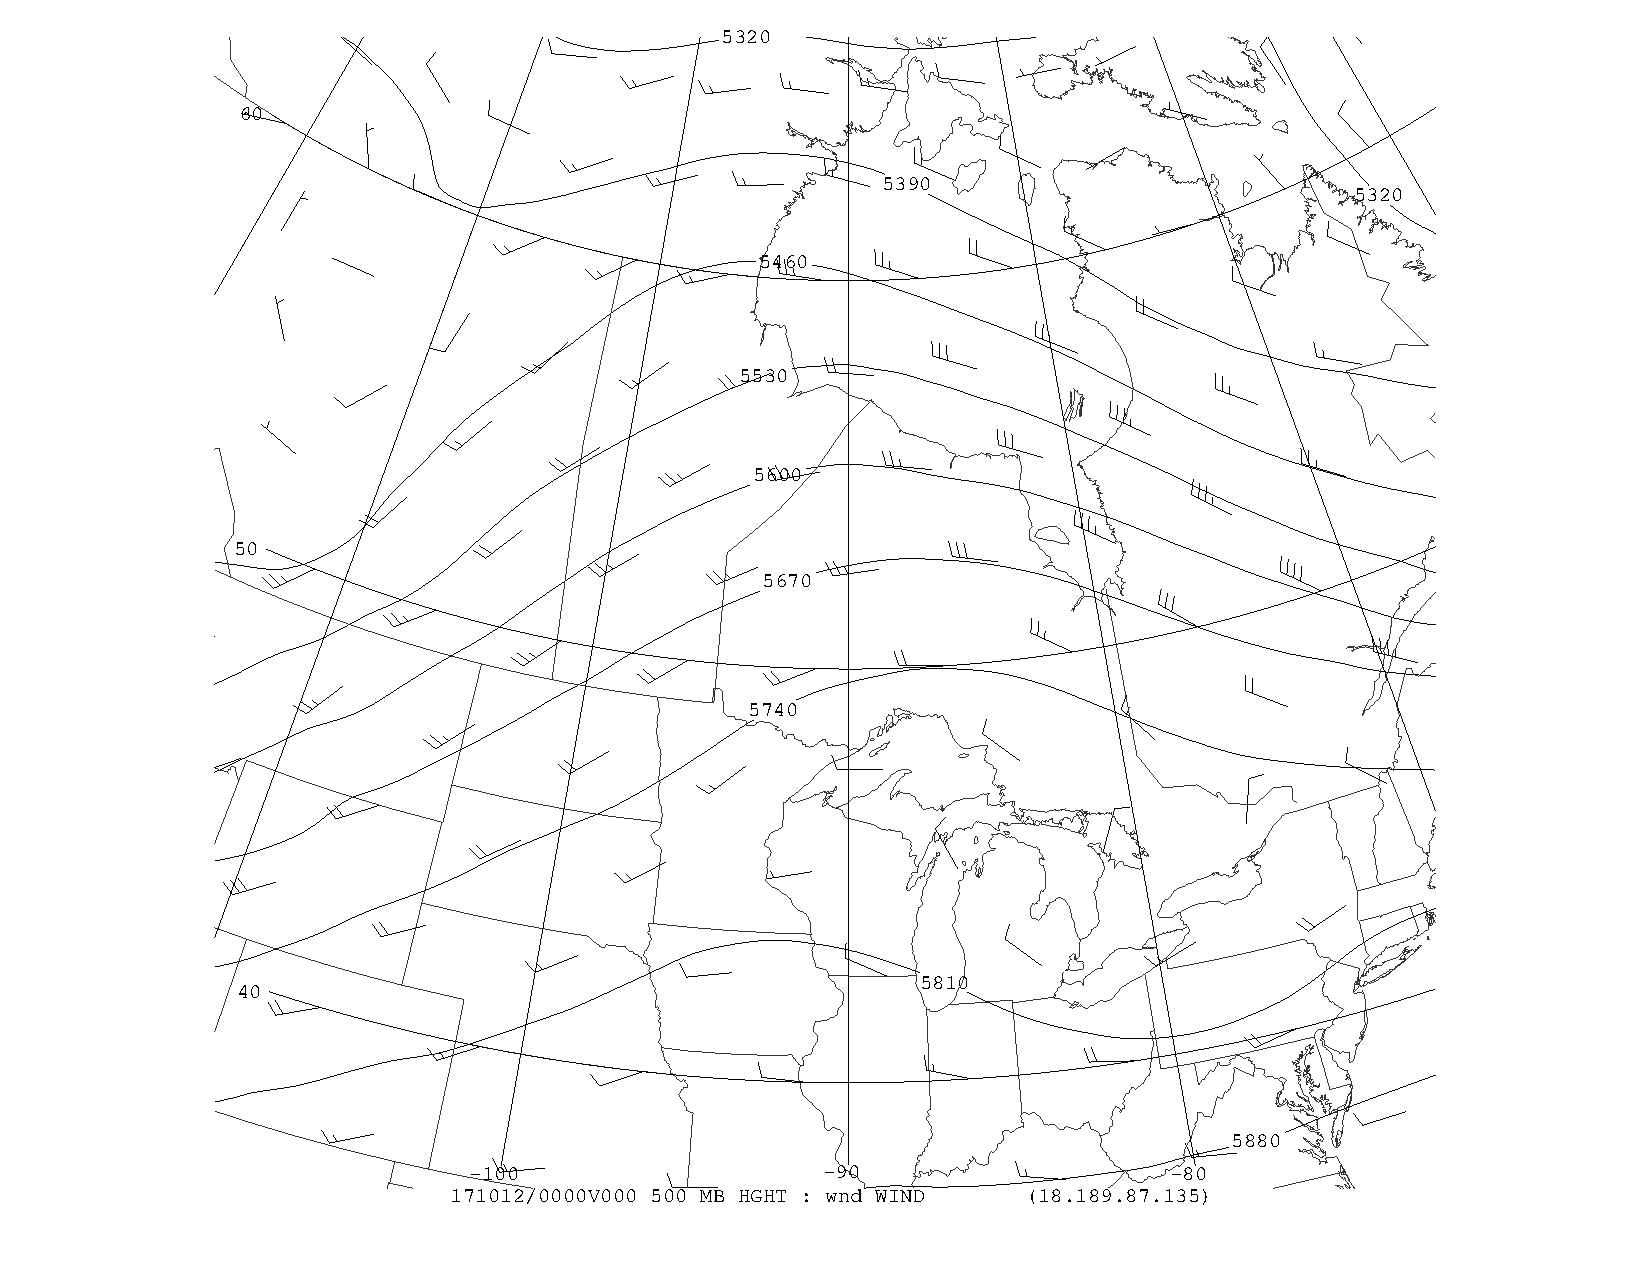
\includegraphics[trim={3.5cm 1cm 3.5cm 0},clip,width=\textwidth]{500hPa_hght_wind_hudson_bay}
	\caption{Geopotential height contour map and wind velocity field at \SI{500}{\hecto\Pa} over the northern United States and Canada on October 12, 2017 0Z.}
	\label{fig:hudson}
\end{figure}

At this location $\phi \approx \SI{57}{\degree N}$ giving a Coriolis parameter of $f = \SI{1.22e-4}{}$. Then approximating the $\partial h/\partial x$ term using a centered finite difference operator, we get that
\begin{equation*}
	\p{h}{y} \approx \frac{\Delta h}{\Delta y} = \frac{\SI{5460}{\m} - \SI{5600}{\m}}{\SI{550}{\km}} = \SI{-2.55e-4}{}
\end{equation*}
where we approximated the distance between the \SI{5460}{\m} and \SI{5600}{\m} geopotential height contours using Google Maps. This gives us an estimated geostrophic wind speed of $u \approx \SI{20.4}{\m/\s}$ (and $v \approx 0$) which agrees closely with the observed westerly wind of \SI{20}{\m/\s} as indicated by the wind barb.

\section{Ageostrophic motion}
If the observed wind pattern is not completely described by geostrophic balance, then any difference between the observed wind and the geostrophic wind may be called the \emph{ageostrophic wind}. We should be able to detect it quite well by looking at atmospheric jets, particularly their entrance and exit through surfaces of constant pressure. Figure \ref{fig:jet} shows a geopotential contour plot and wind velocity field at \SI{200}{\hecto\Pa} over the North Atlantic on October 17, 2017 0Z, while figure \ref{fig:jet_geo} shows the geostrophic wind velocity field and figure \ref{fig:jet_age} shows the ageostrophic wind velocity field.

\begin{figure}[h!]
	\centering
	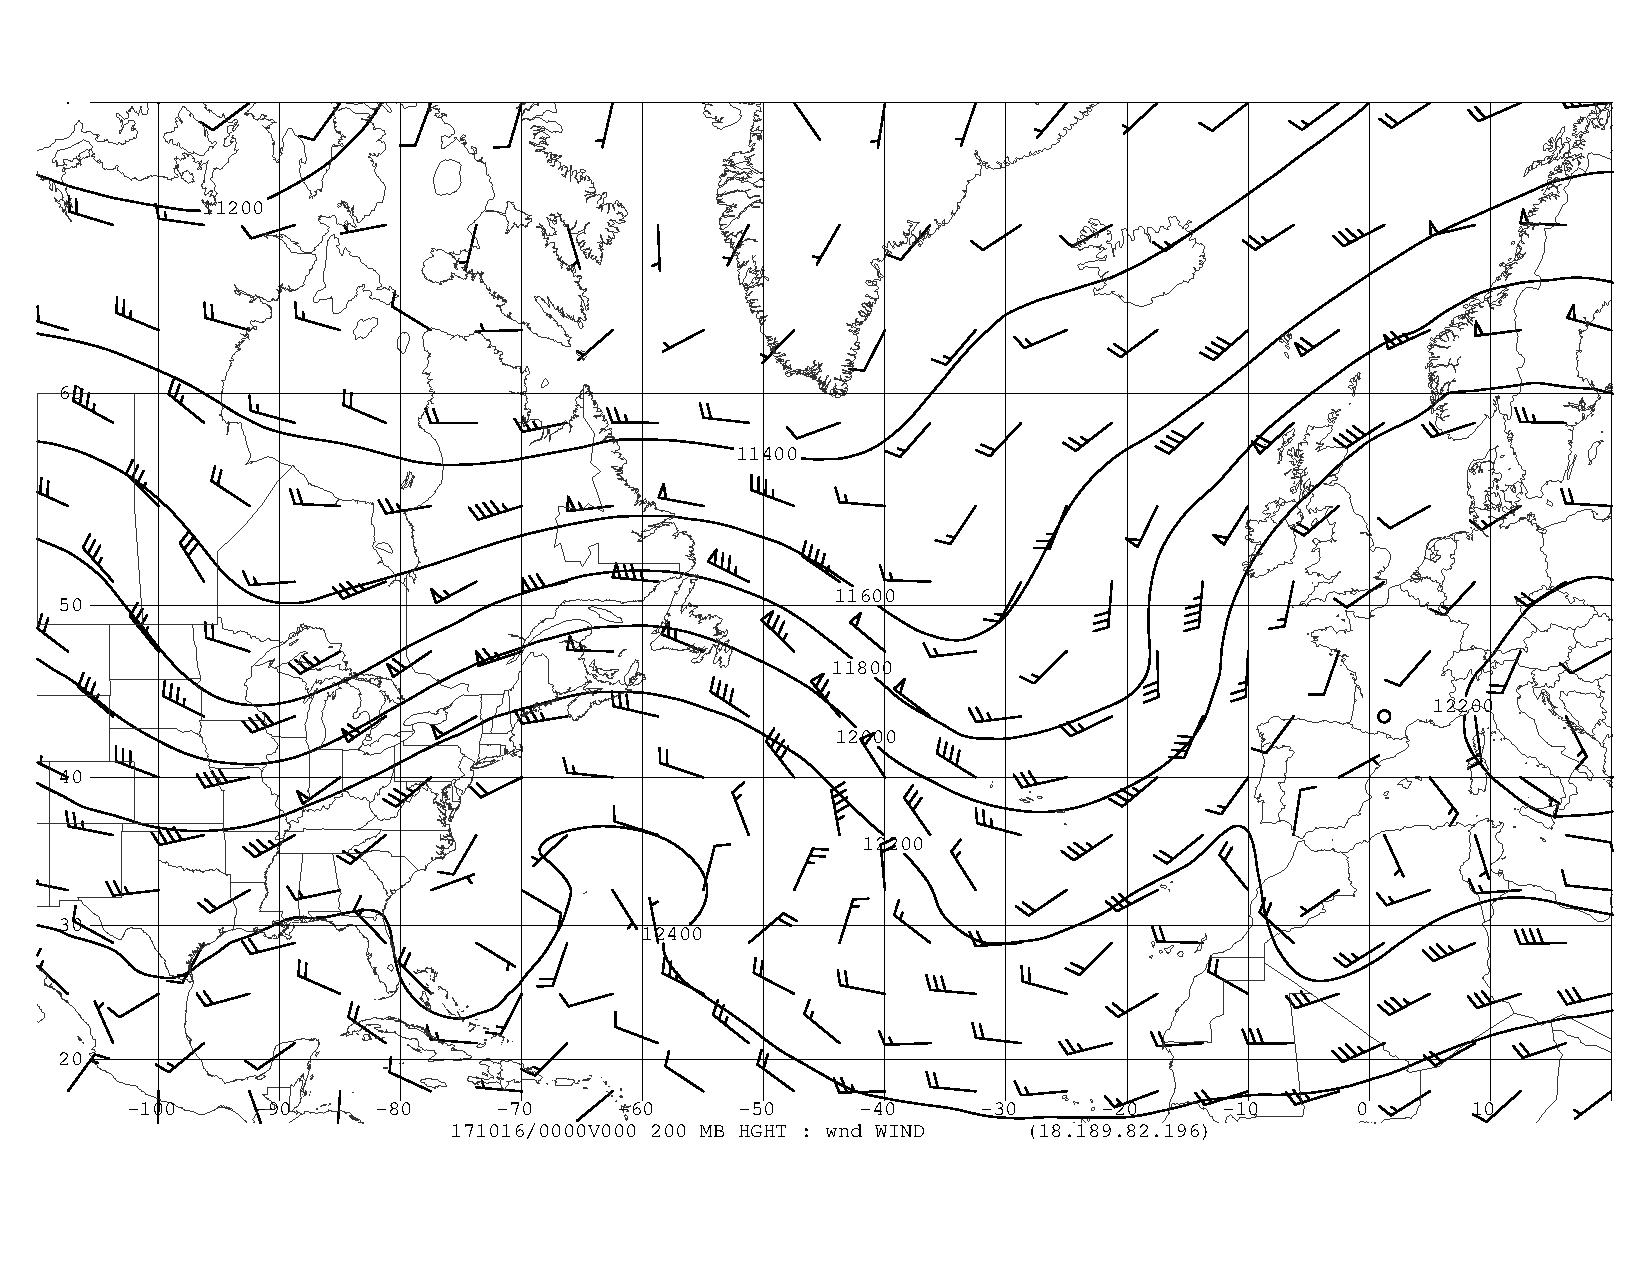
\includegraphics[trim={0.5cm 2cm 0.5cm 0},clip,width=\textwidth]{200hPa_hght_wind_jet_inout}
	\caption{Geopotential contour plot and wind velocity field at \SI{200}{\hecto\Pa} over the North Atlantic on October 17, 2017 0Z.}
	\label{fig:jet}
\end{figure}

\begin{figure}[h!]
	\centering
	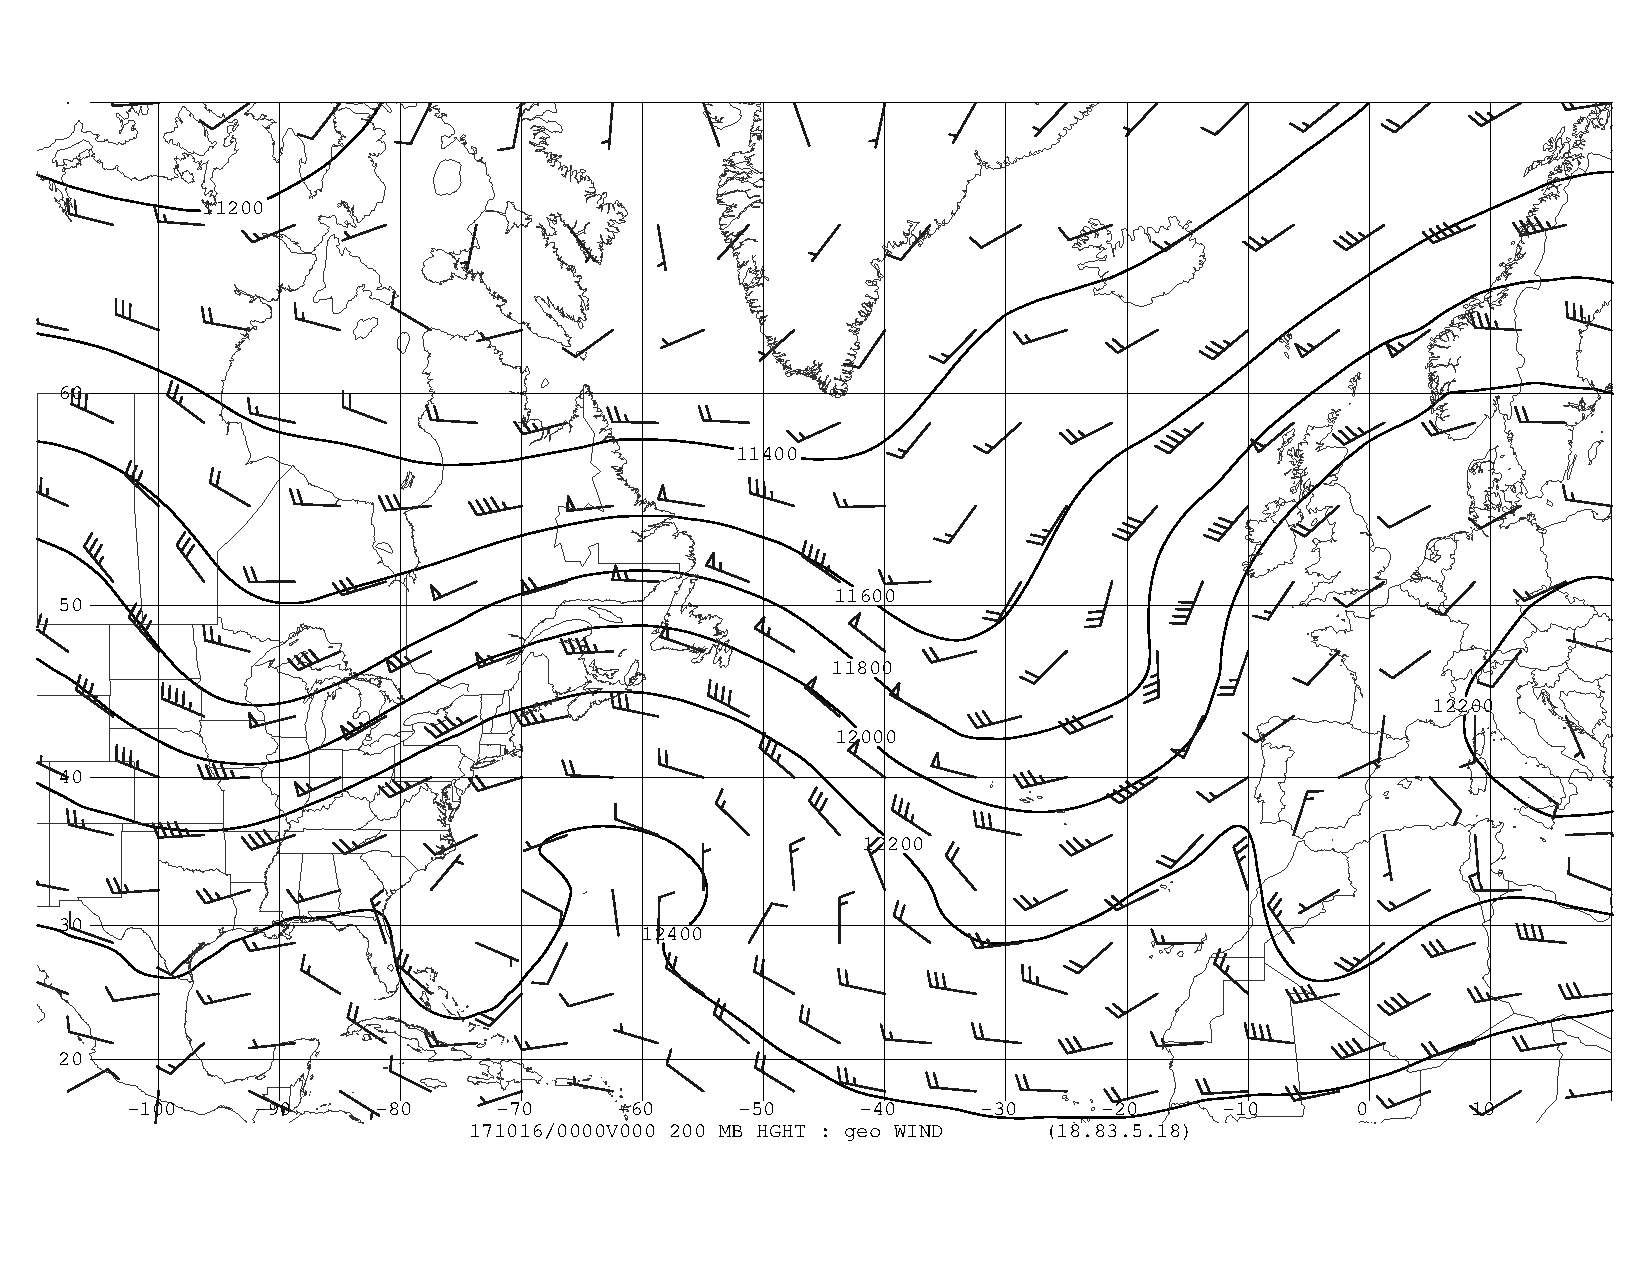
\includegraphics[trim={0.5cm 2cm 0.5cm 0},clip,width=\textwidth]{200hPa_hght_geowind_jet_inout}
	\caption{Geopotential contour plot and geostrophic wind velocity field at \SI{200}{\hecto\Pa} over the North Atlantic on October 17, 2017 0Z.}
	\label{fig:jet_geo}
\end{figure}

\begin{figure}[h!]
	\centering
	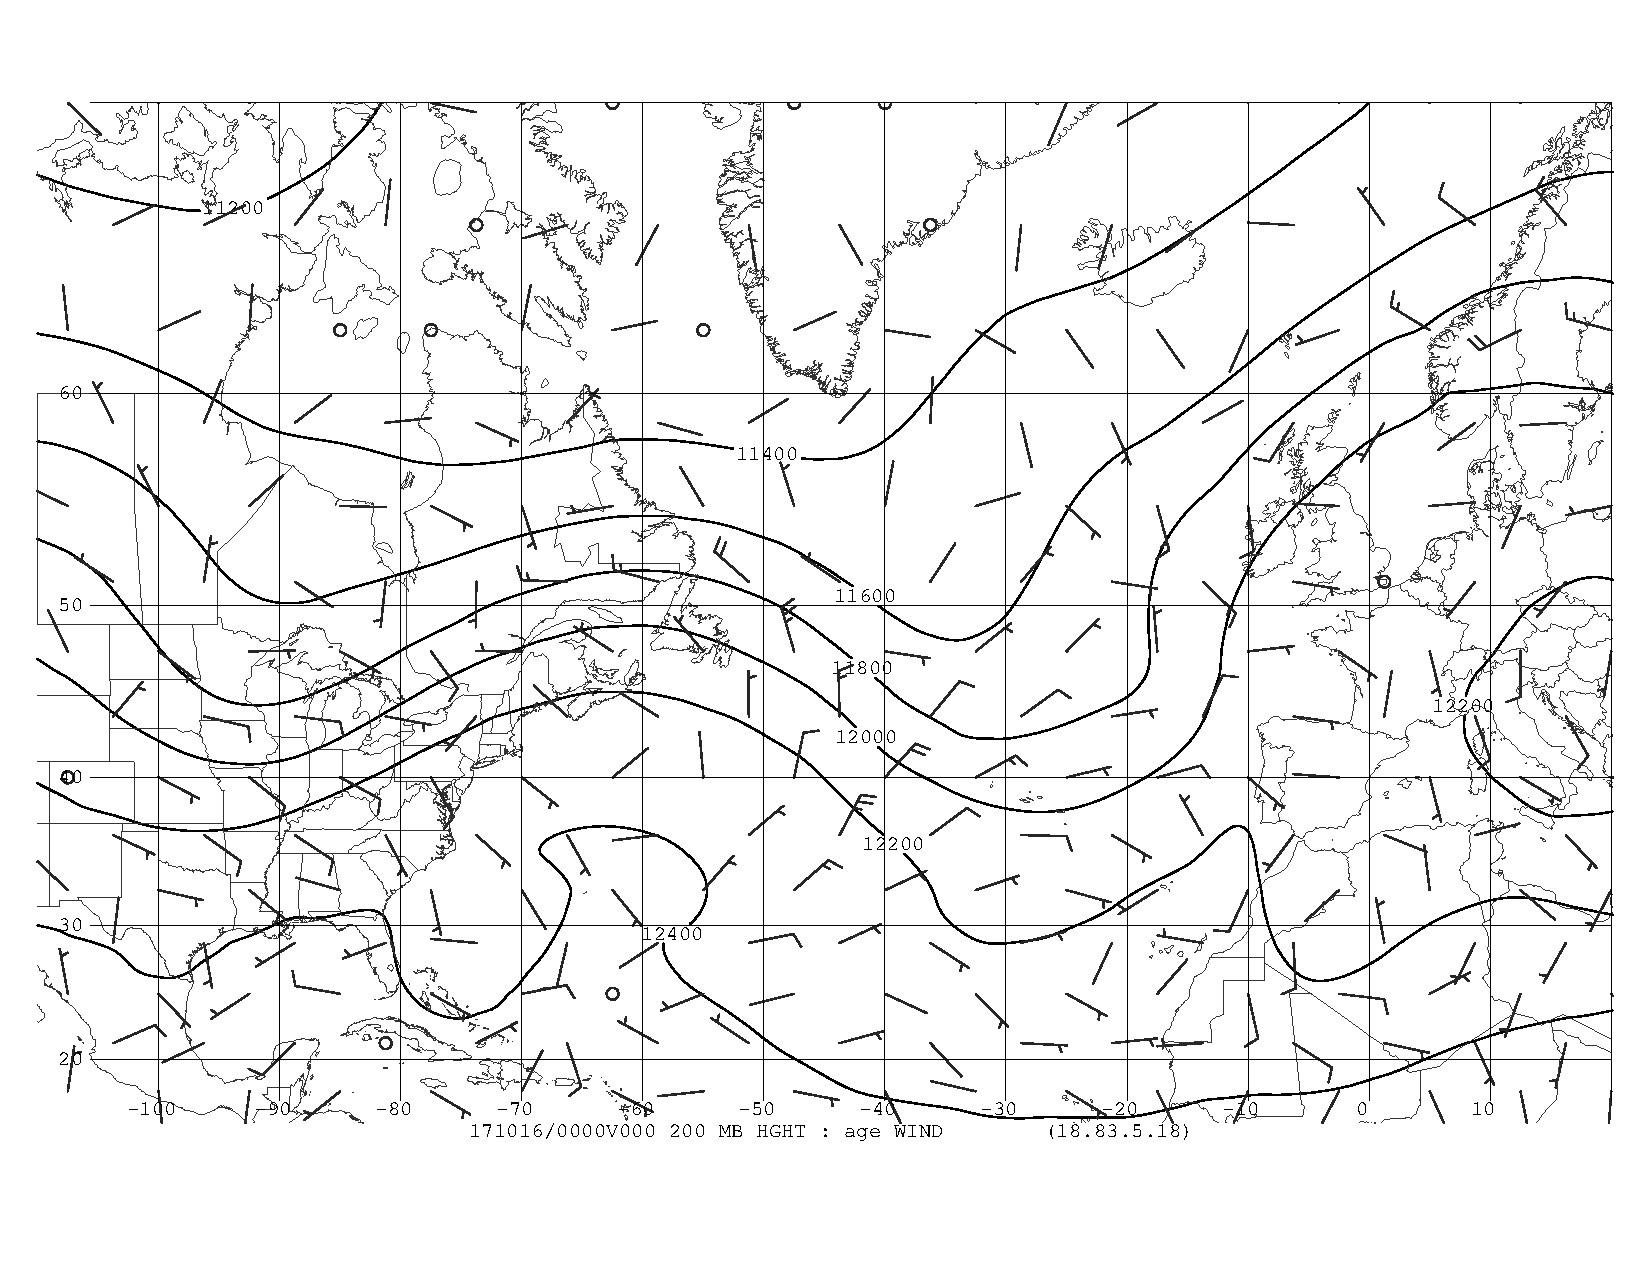
\includegraphics[trim={0.5cm 2cm 0.5cm 0},clip,width=\textwidth]{200hPa_hght_agewind_jet_inout}
	\caption{Geopotential contour plot and ageostrophic wind velocity field at \SI{200}{\hecto\Pa} over the North Atlantic on October 17, 2017 0Z.}
	\label{fig:jet_age}
\end{figure}

\section{Geostrophic and ageostrophic winds in a hurricane remnant}
We will now look at the winds around Hurricane Ophelia, the easternmost Atlantic major hurricane on record, off the coast of Western Europe (Spain, France, Great Britain, and Ireland) on October 16, 2017 as plotted in figure \ref{fig:ophelia}. By this point in time, Hurricane Ophelia has weakened considerably and we refer to it as a hurricane \emph{remnant}. Repeating the same analysis we did over the Hudson Bay, we will calculate the geostrophic wind velocity for a point near the hurricane eyewall or as close as we can get (red oval), a point near the outer rain bands (blue oval), and for a third intermediate point (green oval).

\begin{figure}[h!]
	\centering
	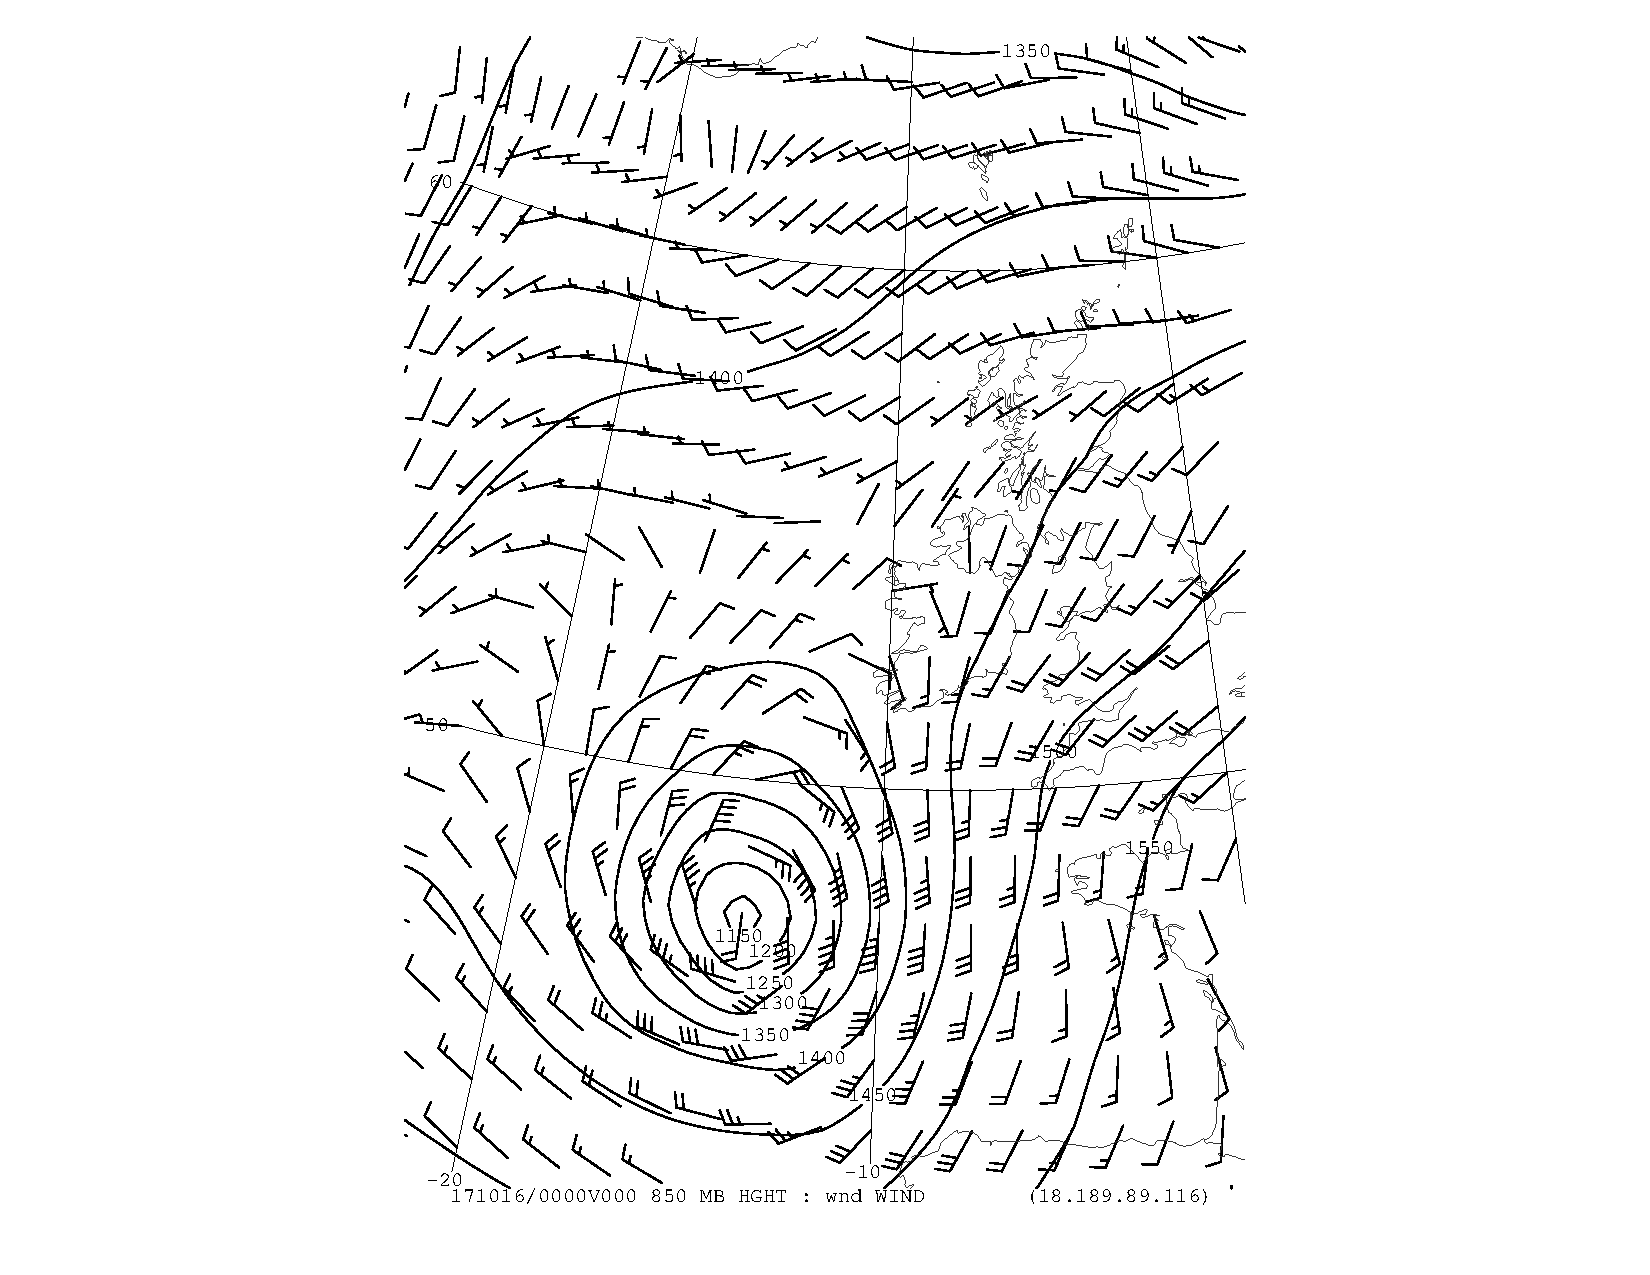
\includegraphics[trim={3.5cm 1cm 3.5cm 0},clip,width=\textwidth]{850hPa_hght_wind_ophelia}
	\caption{Geopotential height contour map and wind velocity field at \SI{850}{\hecto\Pa} off the coast of Western Europe (Spain, France, Great Britain, and Ireland) on October 16, 2017 0Z. The red oval corresponds to a location near the hurricane eyewall, the blue oval to a location near the outer rain bands, and the green oval to an intermediate location, all used for calculations of geostrophic winds and Rossby number.}
	\label{fig:ophelia}
\end{figure}

Near the hurricane eyewall (red oval) and using Eq. \ref{eq:1v} we estimate a northernly geostrophic wind of $v \approx \SI{80}{\m}$ as compared to the wind barb value of \SI{35}{\m} indicating that forces other than the Coriolis force and pressure gradient force are playing a large role in dictating the wind patterns near the hurricane eyewall. In this case the centripetal acceleration due to the hurricane's rotation plays a more significant role and the resultant balance between those three forces is called \emph{gradient balance} and can be represented mathematically in polar coordinates with the hurricane eyewall as the origin as
\begin{equation*}
	\frac{v^2}{r} + fv = g\p{h}{r}
\end{equation*}
and is simply Eq. \eqref{eq:1v} with an extra term corresponding to the centripetal acceleration.

On the outer rain bands (blue oval) and using Eq. \ref{eq:1u} we estimate a westerly geostrophic wind of $u \approx \SI{32}{\m}$ which compares more favorably with the wind barb value of \SI{25}{\m/\s}, however indicating that the centripetal force produced by the hurricane is still rather significant. In between the eyewall and outer rain bands (green oval) and using Eq. \ref{eq:1v} we estimate a southernly geostrophic wind of \SI{50}{\m/\s} which still compares rather favorably with the wind barb value of \SI{45}{\m/\s}.

We can estimate the importance of the centripetal acceleration term by calculating the Rossby number around the hurricane and plotting a Rossby number contour map in figure \ref{fig:ophelia_rossby}. We see a background value below 0.5 for normal conditions far away from the hurricane but near the eyewall it is greater than 2.5 and still above 0.5 near the three ovals we used previously.

\begin{figure}[h!]
	\centering
	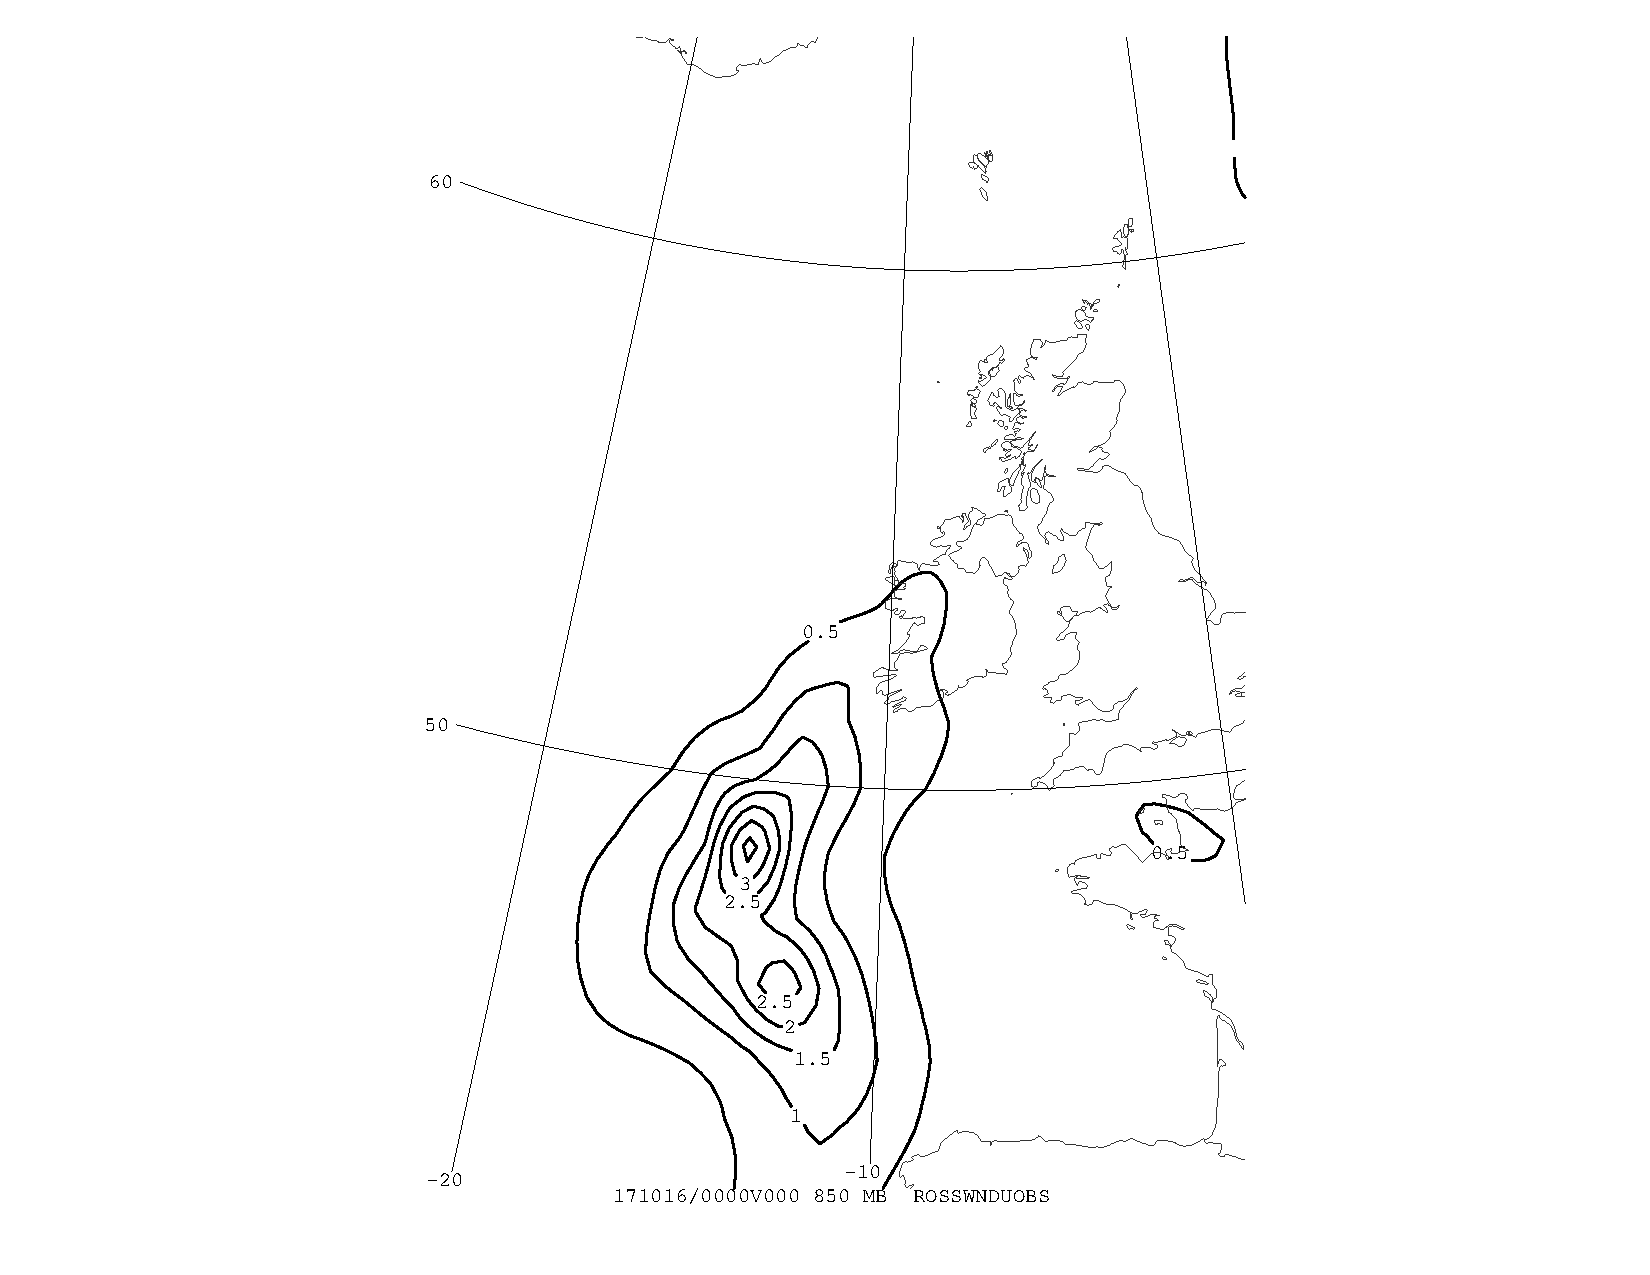
\includegraphics[trim={3.5cm 1cm 3.5cm 0},clip,width=\textwidth]{850hPa_rossby_ophelia}
	\caption{Rossby number contour map around Hurricane Ophelia at \SI{850}{\hecto\Pa} off the coast of Western Europe (Spain, France, Great Britain, and Ireland) on October 16, 2017 0Z.}
	\label{fig:ophelia_rossby}
\end{figure}

%\begin{thebibliography}{9}
%\bibitem{Kalnay}
%Kalnay, E., Kanamitsu, M., Kistler, R., Collins, W., Deaven, D., Gandin, L., Iredell, M., Saha, S., White, G., Woollen, J. and Zhu, Y., 1996. The NCEP/NCAR 40-year reanalysis project. \textit{Bulletin of the American meteorological Society}, 77(3), pp. 437--471.
%\end{thebibliography}

\end{document}